\documentclass{acaces}

\usepackage{wrapfig}

\begin{document}

\title{"\textit{Smart}" Manual Software Parallelisation Assistant}

\author{
Aleksandr~Maramzin\addressnum{1}\extranum{1},
Bj\"{o}rn Franke\addressnum{1}\extranum{2},
Murray Cole\addressnum{1}\extranum{2}
}

\address{1}{
Institute For Computing Systems Architecture, 
Informatics Forum, 
The University of Edinburgh, 
10 Crichton Street, 
Edinburgh, 
UK
}

\extra{1}{E-mail: s1736883@sms.ed.ac.uk}
\extra{2}{E-mail: \{bfranke,mic\}@inf.ed.ac.uk}

\pagestyle{empty}

\begin{abstract}
\quad Since automatically parallelizing compilers have failed to deliver significant performance improvements, programmers are still forced to parallelize legacy software manually for all but some niche domains. Rather than hoping for an elegant silver bullet, we acknowledge the role of a human expert in the parallelization process and develop a \textit{smart} parallelization assistant.\newline\null
\quad In its essence our assistant is yet another application of machine learning techniques to the field of optimizing compilers, which tries to predict the parallelisability property of program loops. We use Seoul National University version of NAS Parallel Benchmarks (NPB) \cite{nasa-parallel-benchmarks}, \cite{snu-npb-benchmarks} hand-annotated with OpenMP parallelisation pragmas to train our ML model. We show that the loop parallelisability classification problem can be successfully tackled with machine learning techniques (using only static code features) achieveing accuracy of around 90\% and outperforming all available baseline random predictors working at an accuracy ranging between 40\% and 70\%.\newline\null
\quad To get a real practical application of our techniques, we integrate our trained ML model into an assistant scheme, designed to mitigate the effects of ineradicable statistical errors and make them less critical. Taking application profile our assistant directs a programmer's efforts by pointing the loops, which are highly likely to be parallelisible and profitable as well. Thus, decreasing the efforts and time it takes to parallelize a program manually. As a side effect our assistant extends the capabilities of Intel C/C++ compiler in the task of parallelism discovery by increasing the amount of parallelism found in SNU NPB benchmarks from 81\% to 96\%.
\end{abstract}

\keywords{ACACES; poster session; software engineering; parallel programming; compilers; static program dependence analysis; loop iterator recognition; machine learning; programmer feedback;}

\section{Introduction}
\quad Since automatically parallelizing compilers have failed to deliver significant performance improvements, programmers are still forced to parallelize legacy software manually for all but some niche domains. Indeed, as our preliminary exploratory experiments showed the effects that Intel C/C++ Compiler (ICC) had brought with its vectorizing and parallelizing transformations to SNU NPB benchmarks ranged from no change to a significant slowdown. Rarely ICC vectorization was able to achieve a tiny speedup, but the former faded in comparison with the speedup of an expertly parallelised SNU NPB OpenMP version. Given these observations we decided to acknowledge the role of a human expert in the parallelization process and develop a \textit{smart} manual software parallelization assistant.\newline\null
\quad Our assistant is based on a ML model, trained to classify program loops as parallelisible or not. We use Seoul National University version of NAS Parallel Benchmarks (NPB) \cite{nasa-parallel-benchmarks}, \cite{snu-npb-benchmarks} hand-annotated with OpenMP parallelisation pragmas to train our ML model. We show that the loop parallelisability classification problem can be successfully tackled with machine learning techniques (using only static code features) achieveing accuracy of around 90\% and outperforming all available baseline random predictors working at an accuracy ranging between 40\% and 70\%.\newline\null
\quad The application of ML techniques to the field of parallelising compilers is not a new endeavour. As the survey of machine learning in optimising compilers \cite{mob-ml} shows there have been numerous successful application attempts. Machine learning can be used for problems ranging from selecting the best compiler flags to determining how to map parallelism to processors. Uneradicable statistical errors inherent to all ML techniques might result in the performance losses here, but do not compromise the ultimate functional correctness of the program being compiled. In this work we step into a potentially dangerous area. False positives (non-parallel loops predicted as parallelisable) can break the program. There is an already published work \cite{fried_ea:2013:icmla} studying the possibility of learning loop parallleisability property. The answer is "yes" and the work reports on a predictive performance (accuracy, recall, precision, etc.) we can achieve. But apart from studying the possibility that work does not step any further to actually find any practical utilisation of loop parallelisability predictor. Moreover, the dataset is highly unbalanced (), which sets the baseline accuracy very high. The authors use dynamic program features.\newline\null
\quad In our work we use static program features for the same loop parallelisability classification problem. We work with a more balanced dataset with richer sources of information our classification labels have been derived from. At the end we harness our trained ML model into a practical application scheme. The scheme has been designed to mitigate the effects of ineradicable statistical errors and make them less critical. Taking application profile our assistant directs a programmer's efforts by pointing the loops, which are highly likely to be parallelisible and profitable as well. Thus, decreasing the efforts and time it takes to parallelize a program manually. As a side effect our assistant extends the capabilities of Intel C/C++ compiler in the task of parallelism discovery by increasing the amount of parallelism found in SNU NPB benchmarks from 81\% to 96\%.

\section{Predicting Parallel Loops}
\label{predicting_parallel_loops}
\quad We pose a \textit{\textbf{supervised machine learning (ML) classification problem}}: create an ML based model and train it to classify loops of Seoul National University (SNU) implementation \cite{snu-npb-benchmarks} of NAS Parallel Benchmarks (NPB) \cite{nasa-parallel-benchmarks} as parallelizable or not.\newline\null
\quad Our work encompasses two technical aspects. First, we need to find a representative set of quantifiable features, which would accurately reflect the parallelisability property of program loops, then we need to select the exact ML training/testing methodology to employ for our problem.\newline\null
\quad Our features and the exact parameters of methodology (automatic feature selection methods, ML models and their hyper-parameter spaces, etc.) have been iteratively tuned with the help of K-fold CV. Predictive accuracy, recall and precision scores were used as the main selection criteria. We used facilities of \textit{scikit-learn} \cite{scikit-learn} Python library for all machine learning related tasks.

\subsection{Feature Engineering}
\label{feature_engineering}
\quad In the task of coming up with a set of loop features we are guided by general program dependence analysis theory \cite{Kennedy:2001:OCM:502981}, exact types of loops present in SNU NPB benchmarks and Intel C/C++ compiler optimisation reports.\newline\null
\quad There is a range of SNU NPB loops, which escape Intel compiler parallelisation for different reasons: indirect array references, unrecognised reductions on array locations, pointers with statically unknown memory locations, etc. But all that range of different reasons is going to ultimately materialise into data and control dependencies present between loop instructions, represented as edges on the Program Dependence Graph (PDG) \cite{Ferrante:1987:PDG:24039.24041} of a loop. To refine our features we conduct a generalised loop iterator recognition \cite{Manilov:2018:GPI:3178372.3179511} analysis on the PDG graph. Figure \ref{fig:pdg} shows an example of a PDG built for a simple loop and visualised with our tool.\newline\null
\begin{figure}
\centering
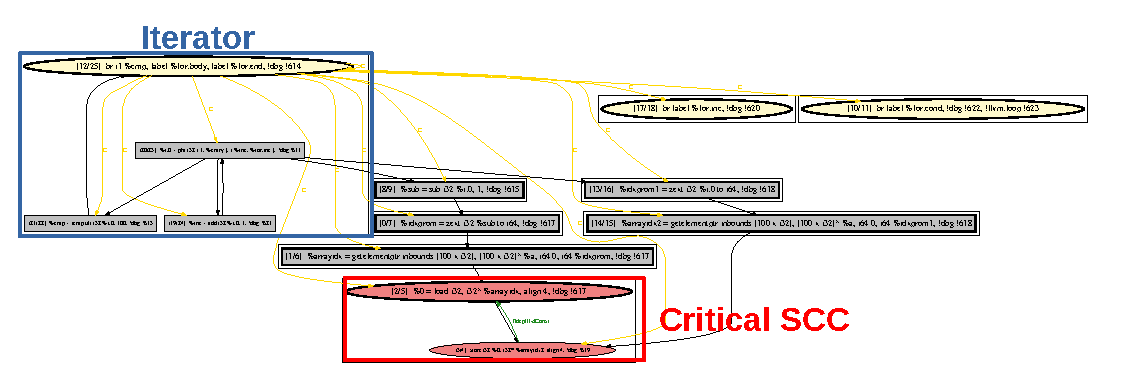
\includegraphics[width=1.0\textwidth]{pdg_example}
\caption{Program Dependence Graph of a simple loop with recognised iterator, regular and critical payload parts. Nodes are LLVM IR instructions, edges are different types of dependencies between them.}
\label{fig:pdg}
\end{figure}
\quad We base our loop features on a static structural properties of PDG. There are 74 different static loop features we use for the ML task. The features are simplistic and defined as different numbers and fractions calculated on a graphs: number of particular LLVM IR instructions (calls, loads, stores, branches, etc.), numbers of various dependence edges (true, anti, output, etc.), sizes of iterators and payloads, etc.

\subsection{Machine Learning Methodology}
\label{ml-methodology}
\quad The final predictive performance we are going to achieve depends not only on the successful choice of loop features, but on the exact training and testing methodology as well. The latter is composed of a number of stages lined up in a pipeline. The pipeline starts with data preprocessing and automatic feature selection (low variance feature elimination, tree based methods, RFECV, etc.) in order to exclude redundant and irrelevant features, which lean to model over-fitting. Then we choose the exact ML model (SVC, DT, RFC, MLP, AdaBoost) to use and tune its hyper-parameters. Typical examples include \textit{C}, \textit{kernel} and $\gamma$ for Support Vector Classifiers (SVC), exact architecture for neural network based models, etc. And finally, we conduct the actual training and testing with standard K-fold and modified Leave-One-Out Cross-Validation (LOOCV)  techniques described in the literature \cite{James:2014:ISL:2517747}. These methods aim at different goals. While K-fold method averages accuracy scores on different data set splits and can be used for feature selection, hyper-parameter tuning and overall predicitve performance estomation, modified LOOCV can be applied against any single SNU NPB benchmark in order to assess our assistant scheme (see section \ref{assistant-scheme}). Table \ref{tab:accuracy} provides the ultimate accuracy we managed to achieve.

\begin{wraptable}{H}{0.5\textwidth}
	\centering
	\begin{tabular}[c]{|p{1.5cm}|p{1.5cm}|p{1.5cm}|p{1.5cm}|}
		\hline
		ML model & accuracy & recall & precision \\
		\hline
		constant & 70.32 & 100 & 70.32\\
		\hline
		uniform & 46.27 & 41.50 & 69.79\\
		\hline
		SVC & 90.04 & 95.24 & 91.06 \\
		\hline
		AdaBoost & 86.96 & 92.92 & 89.06 \\
		\hline
		DT & 84.36 & 89.57 & 87.90 \\
		\hline
		RFC & 86.65 & 93.22 & 88.47 \\
		\hline
		MLP & 89.40 & 93.77 & 91.39 \\
		\hline
	\end{tabular}
	\caption{Average predictive performance for different ML models measured with a K-fold CV method on the whole set of 1415 SNU NPB loops.}
	\label{tab:accuracy}
\end{wraptable}

\section{Manual Software Parallelisation Assistant}
\label{assistant-scheme}
\quad Achieving high prediction accuracy is not enough. We need to find a way to utilise our work practically. Due to statistical nature inherent to all ML techniques, it is impossible to completely eliminate all prediction errors. While false negative mispredictions might just miss available parallelisation opportunities and lose some performance, false positive mispredictions can break the program and are the most critical in the context of our ML problem. For that reason we propose assistant schemes that leave the question of final parallelisation up to a programmer to decide.\newline\null
\quad Our predictor is capable of discovering additional parallelisation opportunities, which escape the conservative analysis of Intel compiler. For SNU NPB benchmarks we increse the amount of discovered parallelism from 81\% to 96\%. But not all parallel loops have to be parallelised. We are interested only in the loops, which take significant application runtime fraction and thus directly affect overall performance. Our assistant takes an application profile and orders an application loops according to their running time. But not all long running loops are parallelisable. We multiply loop running times on the function (shifted sigmoid) of loop parallelisability probability extracted out of ML model and get an improved ranking. Figure \ref{ranking} illustrates the principle.
\begin{figure}
\centering
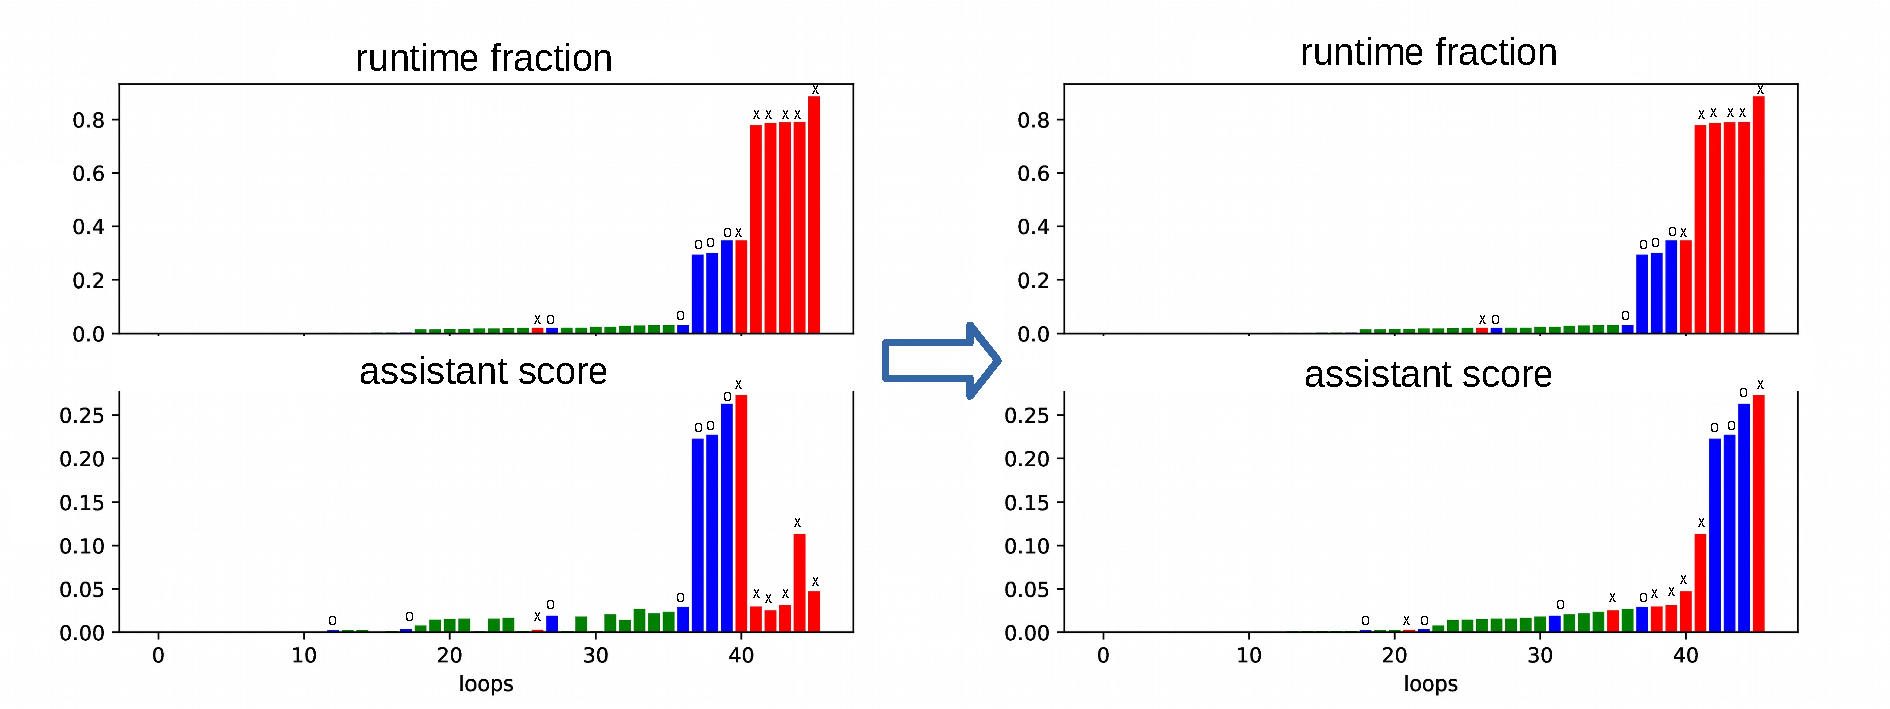
\includegraphics[width=1.0\textwidth]{ft_ranking}
\caption{Illustration of loop ranking transformation.}
\label{ranking}
\end{figure}

\section{Evaluation}
\label{evaluation}
\quad Parallelising the program by following the reorded list of program loops, a programmer can get to the best achievable performance faster. Figure \ref{convergence} illustrates the process.   
\begin{figure}
	\centering
	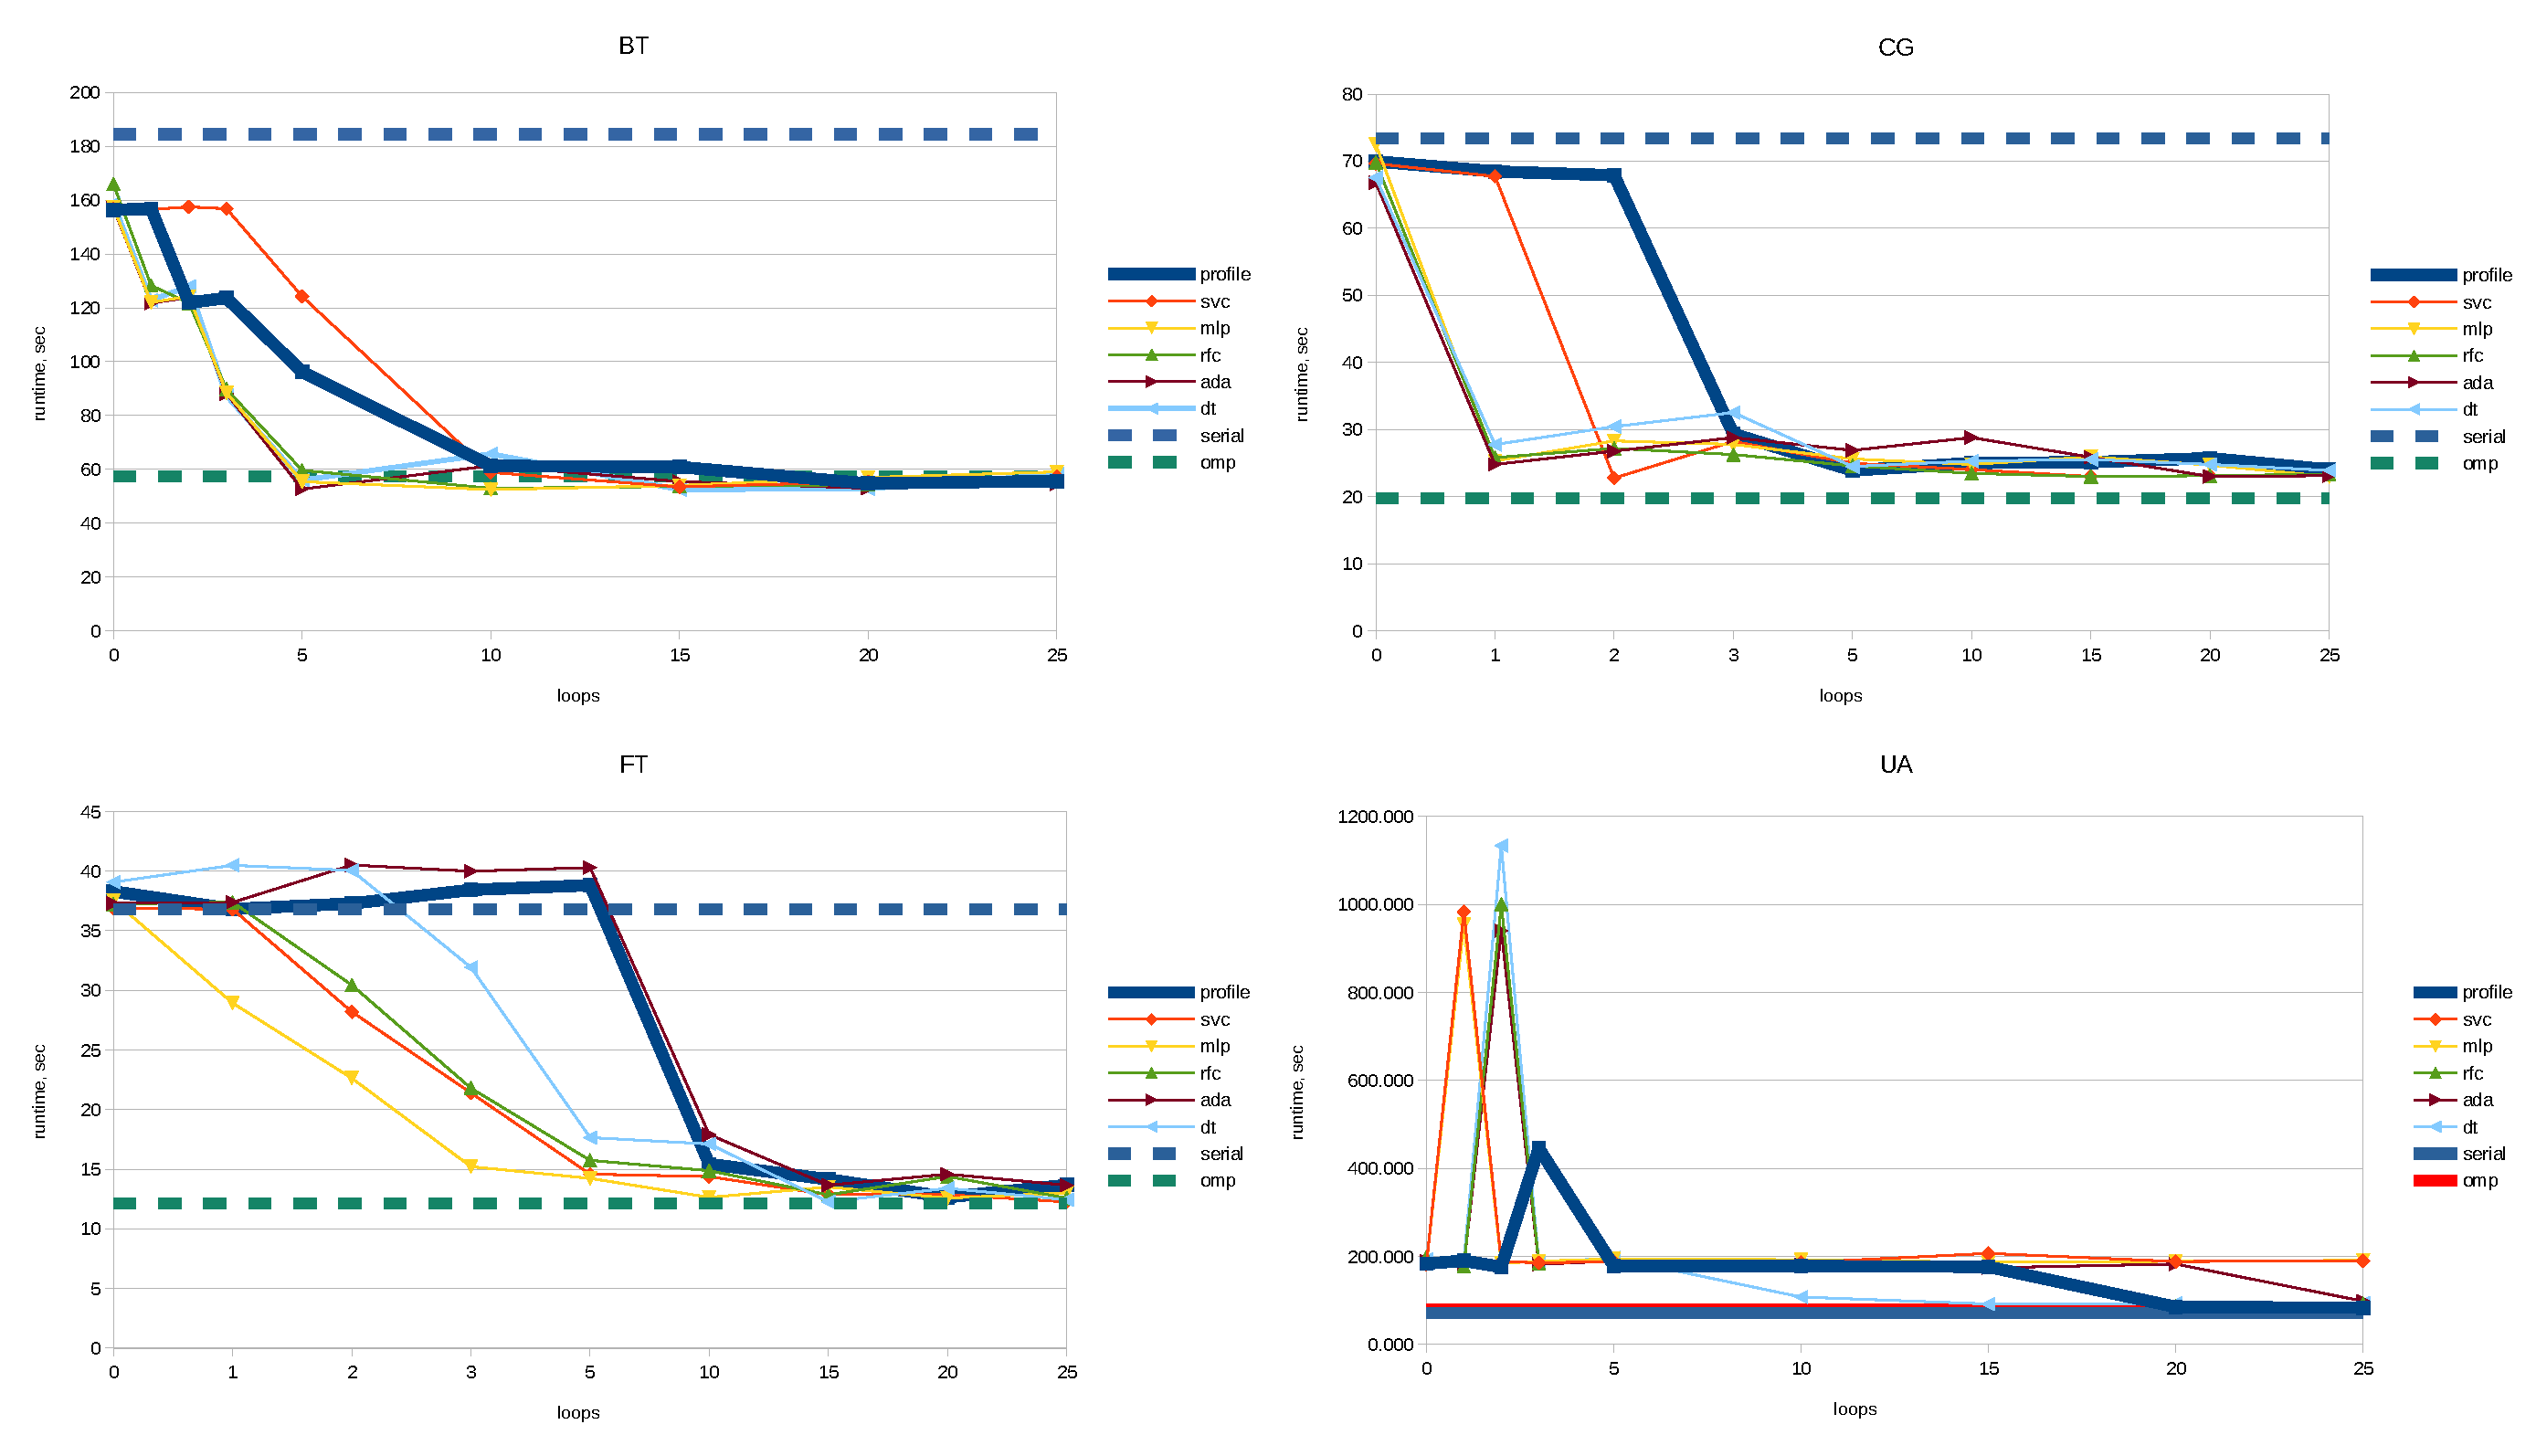
\includegraphics[width=1.0\textwidth]{parallelisation_acceleration}
	\caption{Illustration of a faster convergence to the maximum achievable parallel software performance.}
	\label{convergence}
\end{figure}

\bibliography{guide}

\end{document}

